\section{Analysis and Design}
\begin{comment}
If your project involves designing a system, give a
good high-level overview of your design.\\ \newline \noindent In many projects, the final design is different from
that originally envisaged. If the differences are
interesting, write about them, and why the changes
were made. Discoveries during the project may have changed the direction of work, or invalidated prior
work, in which case you get credit for the design
process, if it is principled, as well as the end product.\\ \newline \noindent If your design was not implemented fully, describe
which parts you did implement, and which you didn't.
If the reason you didn't implement everything is
interesting (eg it turned out to be difficult for
unexpected reasons), write about it.\\ \newline \noindent Note that the Project Report is written at the end of
project work and must describe the project work, but
need not do this chronologically. Often the best
description of design, in retrospect, is far from the
way in which you developed it. Where the evolution
of ideas is interesting or relevant it can be described,
as above, but otherwise the order in which things
were done need not be documented.\\ \newline \noindent The Examiners are just as interested in the
engineering process you went through in performing
your project work as the results you finally produced.
So make sure your report identifies when design
choices have to be made, what were the possibilities,
and why you made the particular choices and
decisions that you did. They are looking for principled
rational arguments and for critical assessment.
Engineering involves trade-offs and the reasons for a
design decision may be various, and may in some
cases be out of your control. Explicit understanding of
this, and the ability to communicate it, is important.
\end{comment}

In this chapter, the aims are to:

\begin{itemize}
    \item Provide a high-level overview of the design of the system to estimate blood pressure values from PPG signals
    \item Describe the specifications of each block of the system
    \item Discuss any changes or justifications for design choices made for the system blocks where appropriate
\end{itemize}

\subsection{High Level overview of proposed design}

\begin{itemize}
    \item Block diagram of ALL STAGES
    \item Just intro paragraph, based directly off of literature review findings
    \item Then go into sub chapters for each block
\end{itemize}

\begin{figure}[H]
    \centering
    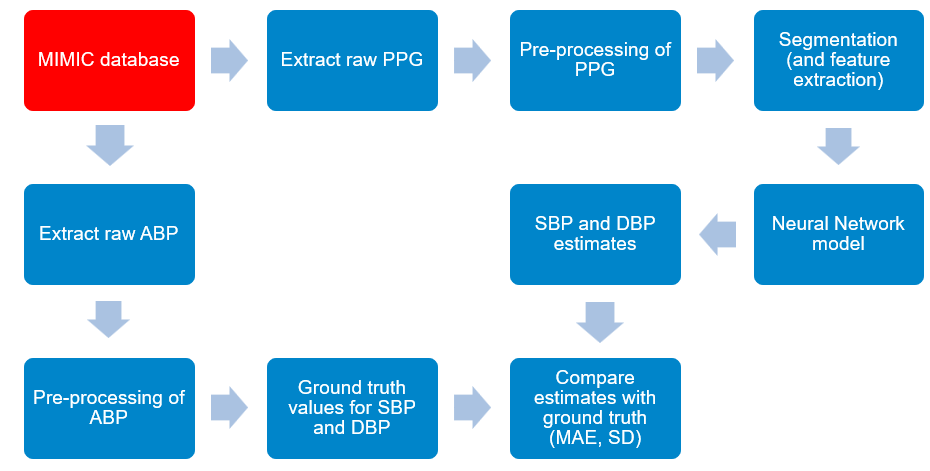
\includegraphics[width=15cm,height=15cm,keepaspectratio]{AnalysisDesign/blockDiag.png}
    \caption{High-level block diagram of blood pressure cuffless estimation from PPG}
    \label{blockdiag}
\end{figure} 

\subsection{Choice of dataset}
\textcolor{red}{Give a better explanation of the dataset you're using. Age range, gender split, any medical conditions.. This can all be found in the dataset website or the relevant papers linked to the dataset.}
As previously discussed in the literature review in Chapter 2, the chosen dataset is the 
Medical Information Mart for Intensive Care (MIMIC) dataset. \textcolor{red}{Did you? I must have overlooked it.} The MIMIC Database 
includes data recorded from over 90 ICU patients. The data in each case include 
signals and periodic measurements obtained from a bedside monitor as well as clinical 
data obtained from the patient's medical record. The recordings vary in length; almost 
all of them are at least 20 hours, and many are 40 hours or more \textcolor{red}{If you know how many, state it. Don't be chatty.}. In all, the database 
contains nearly 200 patient-days of real-time signals and accompanying data \cite{Moody1996}.
\textcolor{red}{I don't understand.. You say there are over 90 ICU patients (again state the exact number because it is known). So where do the 200 come from? (again can't be nearly 200.. Be exact.) - Did you use all 90 or 200 patients data. Everything you write in your methods needs to be clear for someone to repeat exactly what you have done. This will also help us review your code and run it to produce the exact same results you will be showing in the report.}


\subsection{Choice of programming language}
Python is used as the sole programming language for this project. Python has a wide 
variety of easy to use and powerful libraries \cite{Python}. The scientific libraries from Python 
that are used for this project are \texttt{numpy} \cite{numpy} and \texttt{pandas} \cite{pandas}. In addition, the 
machine learning libraries used are \texttt{tensorflow} \cite{tensorflow}, \texttt{keras} \cite{keras} and \texttt{scikit-learn} \cite{scikit}. 
In addition the \texttt{heartpy} \cite{heartpy} and \texttt{wfdb-python} \cite{wfdb} packages were installed, which are libraries of 
tools for reading, writing, and processing Waveform-Database (WFDB) signals and annotations. \\ \newline \noindent MATLAB was also 
considered as a potential programming language to use, due to it having a wide range of 
signal processing and machine learning add-on toolboxes. However Python has been shown 
to offer a wider set of choices in graphics packages and toolsets, such as 
through \texttt{matplotlib} \cite{matplotlib}, and it also produces more compact and readable 
code.

\subsection{Extraction of raw ABP signal data}
JUST DESCRIBE HERE! DONT SAY HOW IT IS DONE, JUST SAY WHY WHERE NEEDED!
\begin{itemize}
    \item Use heartpy library (hp.process)
    \item Despite being measured using gold-standard invasive, still needs preprocessing. TALK ABOUT ALL STEPS!
\end{itemize}

\subsection{Extraction of raw PPG signal data}

\subsection{Pre-processing of PPG}
\begin{itemize}
    \item hp.process
    \item Butterworth filter
    \item Z-normalisation
\end{itemize}

The $Z$-score normalisation equation is applied to the PPG signal, 
\begin{equation}
    Z_{i} = \frac{(PPG_{i} - \mu_{PPG_i}) }{\sigma_{PPG_i}}
\end{equation} \noindent where $Z_{i}$ is the $Z$-score normalised PPG signal for a particular window $i$, 
$PPG_{i}$ is the raw PPG signal, $\mu$ is the mean of the PPG signal and $\sigma$ is the standard deviation.


\subsection{Feature extraction}

\subsection{Proposed Transformer model}

\subsection{Error metrics}
The two considered error calculations used in this experimentation are the Mean Absolute Error 
(MAE) and Root Mean Square Error (RMSE). They are defined by the following equations, 
\begin{align}
    MAE &= \frac{1}{N} \sum_{i=1}^N \lvert a_{i_{M}} - b_{i_{M}} \rvert \\
    RMSE &= \frac{1}{N} \sqrt{\sum_{i=1}^N \lvert a_{i_{M}} - b_{i_{M}} \rvert^2}
\end{align}\noindent In the context of BP estimation, $b_{i_{M}}$ and $a_{i_{M}}$ represent the true 
value and BP estimate respectively for the $M$th element of the time sequence.
